\chapter{Introducción}
\label{chap:intro}

\drop{A}{ctualmente}, existen numerosos avances en lo que a <<nuevas tecnologías>> se refiere y cada vez disponemos de más dispositivos con los que comunicarnos y estar en contacto con amigos, familiares o conocidos en todo momento. Estos avances amplían las formas y posibilidades de comunicación que se encuentran presentes en todos los ámbitos y han modificado la forma de relacionarse, siendo el educativo uno de estos ámbitos. Por ejemplo, antes se recurría al reparto de una circular que los alumnos tenían que hacer llegar a los padres en la que se anunciaban determinados eventos o se escribía una nota en la agenda de algún estudiante para que la entregase firmada al día siguiente si no había hecho los deberes asignados o había ocurrido algún percance durante la jornada escolar. Hoy en día, se usa el correo electrónico para comunicarse con los padres con el fin de establecer una comunicación más directa con estos.

Cercana al correo electrónico existe una plataforma perteneciente a la comunidad autónoma de Castilla-La Mancha llamada <<Papás 2.0>> (Figura \ref{fig:papas20}), que se encuentra más enfocada al sector educativo. Se trata de una plataforma educativa perteneciente a la Consejería de Educación, Cultura y Deportes de la \acf{JCCM} que facilita la gestión administrativa y establece una vía de comunicación entre los centros educativos y las familias, ofreciendo información relevante a los padres \cite{JCCM2017}. Además, permite llevar un seguimiento sobre las tareas, trabajos, controles, exámenes, faltas de asistencia y fechas de entrega \cite{JCCM2010}.

\begin{figure}[!h]
	\begin{center}
		
\includegraphics[width=0.4\textwidth]{/logo_papas_20}
		\caption{Logotipo de <<Papás 2.0>>}
		\label{fig:papas20}
	\end{center}
\end{figure}

\newpage

Papás 2.0 ofrece una serie de características que pueden resultar de gran valor para los padres, siendo las siguientes las más destacadas:

\begin{itemize}
	\item Visualizar los profesores que dan clase a los hijos con sus datos y posibilidad de escribir un mensaje directamente a cualquiera de ellos.
	\item Consultar las citas concertadas con los profesores, junto con la fecha, hora y motivo de la visita.
	\item Consultar el horario escolar.
	\item Consultar las faltas de asistencia, con la posibilidad de ser notificado vía \acf{SMS} o correo electrónico. Del mismo modo, se podrá registrar con anterioridad una notificación cuando se sepa que el hijo va a faltar a ciertas sesiones de clase.
	\item Consultar trabajos y tareas de cada hijo, así como ver las fechas de los exámenes, sus notas del curso y su trayectoria escolar.
	\item Envío y recepción de mensajes mediante grupos, pudiendo adjuntar archivos de tamaño no superior a 1 \acf{MB} por archivo y de un máximo de 3 \acs{MB} en total si se envía más de un archivo.
\end{itemize}

A pesar de que esta aplicación es de gran utilidad por las funcionalidades y facilidades que ofrece tanto a padres como a personal docente, se trata de una plataforma más cercana al correo electrónico que a una aplicación de mensajería instantánea, donde las personas sí que se comunican en tiempo real. En este caso, los \textit{smartphones} tienen especial relevancia puesto que se trata de dispositivos desde los que se puede acceder a casi cualquier servicio ya que se encuentran permanentemente conectados a Internet. Por tanto, normalmente no se espera a tener un ordenador cerca para comunicarse con otras personas, sino que se hace uso directamente del teléfono móvil y de sus aplicaciones. Teniendo esto en cuenta, los profesores podrían comunicarse en tiempo real con los padres y estos pueden aportar algún tipo de \textit{feedback} en un corto periodo de tiempo.

Aunque existen diversas soluciones para la comunicación entre los padres y el centro en el que se encuentren sus hijos y estas aportan numerosos beneficios a la comunidad educativa, muchas veces se pueden producir situaciones poco deseables derivadas, por ejemplo, de determinados malentendidos cuando se hace uso de la mensajería instantánea. Esto se debe a que se crean grupos de chat en los que el centro tiene poco o nada que ver, no se encuentran convenientemente controlados y, con el tiempo, puede producirse una desvirtuación de la finalidad original.

\newpage

Un ejemplo de esa desvirtuación es el siguiente caso, donde un grupo de madres se negaba a llevar a sus hijos al colegio debido a que a la clase de estos acudía un niño que sufría síndrome de Asperger. Sucedió en Buenos Aires, Argentina, y pronto se dio a conocer en Internet.
En las capturas de la conversación (Figura \ref{fig:whatasper}) se puede ver cómo las madres se alegran de que este chico fuera cambiado de clase. <<Una buenísima noticia>>, según indicaba una de las integrantes \cite{Vanguardia2017}.

\begin{figure}[!h]
	\begin{center}
		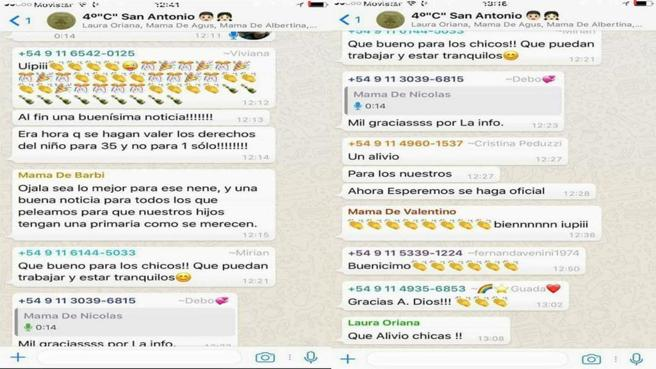
\includegraphics[width=0.7\textwidth, height=0.6\textwidth]{/whatsapp_asperger}
		\caption{Captura conversación inadecuada}
		\label{fig:whatasper}
	\end{center}
\end{figure}

Más allá de los problemas que puedan surgir entre los padres, los grupos pueden llegar incluso a dañar a los propios hijos. Esto puede suceder puesto que hay padres que comparten el trabajo realizado en casa para que otros niños o padres puedan beneficiarse de ello. Esta práctica puede repercutir en un mal aprendizaje del niño y, por tanto, en una disminución de su rendimiento escolar. Otro ejemplo de uso no apropiado es que se pueden llegar a compartir fotos de los regalos colocados debajo del árbol en la época navideña \cite{Alias2017}, como si se tratara de grupos informales. Por todo esto se debe establecer de manera firme y consensuada la figura del administrador del grupo, que será quien se encargue del cumplimiento y gestión de las normas para que la relación y saber estar de los padres no se quede únicamente en el trato presencial sino que se extrapole a las nuevas soluciones digitales.

Otro caso sucedió también en Argentina y es el de una madre que mandó una carta a una periodista explicando cómo, a raíz de abandonar el grupo de madres, estas la tratan de una manera diferente. Esta decisión fue tomada puesto que en dicho grupo se hablaba demasiado, llegando a ser <<insoportables>>, decía la madre \cite{Consuelo2017}.

\newpage

Las bondades de la mensajería instantánea son muy amplias y bien conocidas aunque, como en todo, se debe tener mesura en su uso y cierto control, sobre todo si se trata de temas más sensibles como los que se encuentran relacionados con los hijos. Por eso, en este \acs{TFG} se plantea el desarrollo de una aplicación enfocada al sector educativo que evite, en la medida de lo posible, problemas como los descritos anteriormente.

\section{Estructura de la Memoria}
A continuación, se detalla la estructura de este \acs{TFG}:

\begin{definitionlist}	
	\item[Capítulo \ref{chap:intro}: \nameref{chap:intro}]
	En este primer capitulo se ha realizado una breve introducción al ámbito en el que se desarrolla este trabajo, junto con la presentación de la plataforma educativa \mbox{<<Papás 2.0>>}, así como algunos ejemplos del mal uso de las aplicaciones de mensajería instantánea.
	
	\item[Capítulo \ref{chap:objetivos}: \nameref{chap:objetivos}]
	Se exponen tanto el objetivo principal del trabajo como los objetivos específicos que se deberán cumplir para lograr la consecución del mismo.
	
	\item[Capítulo \ref{chap:antecedentes}: \nameref{chap:antecedentes}]
	Este capítulo está destinado al estudio de las soluciones de mensajería instantánea que se pueden encontrar en el mercado, realizando una comparación de las características de dos de las aplicaciones más utilizadas, WhatsApp y Telegram.
	
	\item[Capítulo \ref{chap:metodologia}: \nameref{chap:metodologia}]
	En este capítulo se exponen las metodologías seguidas a lo largo del desarrollo del \acs{TFG}. Se detalla la metodología de gestión de proyectos y la metodología de desarrollo de software utilizadas.
	
	\item[Capítulo \ref{chap:resultados}: \nameref{chap:resultados}]
	En este capítulo se muestran los resultados obtenidos teniendo en cuenta los objetivos planteados.
	
	\item[Capítulo \ref{chap:conclusiones}: \nameref{chap:conclusiones}]
	Por último, se expondrán las conclusiones obtenidas y los posibles trabajos futuros a realizar sobre el presente \acs{TFG}.
\end{definitionlist}

% Local Variables:
%  coding: utf-8
%  mode: latex
%  mode: flyspell
%  ispell-local-dictionary: "castellano8"
% End: